\documentclass[11pt,a4paper]{article}

\usepackage[T1]{fontenc}
\usepackage{lmodern}
\usepackage[margin=0.95in]{geometry}
\usepackage{amsmath,amssymb,amsthm,mathtools}
\usepackage{booktabs}
\usepackage{graphicx}
\usepackage{xcolor}
\usepackage{microtype}
\usepackage{enumitem}
\usepackage[colorlinks=true,linkcolor=blue!60!black,citecolor=teal!60!black,urlcolor=blue!60!black]{hyperref}

\theoremstyle{plain}
\newtheorem{theorem}{Theorem}[section]
\newtheorem{corollary}[theorem]{Corollary}
\newtheorem{proposition}[theorem]{Proposition}
\newtheorem{lemma}[theorem]{Lemma}
\theoremstyle{definition}
\newtheorem{definition}[theorem]{Definition}
\newtheorem{remark}[theorem]{Remark}

\newcommand{\Ftwo}{\mathbb{F}_2}
\newcommand{\Q}{\mathbb{Q}}
\newcommand{\R}{\mathbb{R}}
\newcommand{\C}{\mathbb{C}}
\newcommand{\SZ}{\mathcal{S}_Z}
\newcommand{\SX}{\mathcal{S}_X}
\newcommand{\KZ}{\mathcal{K}_Z}
\newcommand{\wt}{\operatorname{wt}}
\newcommand{\supp}{\operatorname{supp}}
\newcommand{\Tr}{\operatorname{Tr}}

\title{\textbf{Universal Even--Odd Coherent-Error Parity Dichotomy, Swap-Point Criticality, and Exact-$\mathbb{Q}$ Decoding Certificates for CSS Quantum Codes}}

\author{Lluis Eriksson\thanks{Independent researcher (Sweden). Prepared with AI assistance (Google Antigravity). Code, Lean~4 proofs, and exact-$\Q$ certificates: \url{https://github.com/lluiseriksson/coherent-css-dichotomy} (MIT license).}}

\date{November 2026}

\begin{document}
\maketitle

\begin{abstract}
Uniform coherent $Z$-rotations $U(\theta) = \bigotimes_{j=1}^{n} e^{i\theta Z_j}$ induce non-Pauli logical channels whose optimal recovery and finite-size scaling differ sharply from Pauli-twirled stochastic phase-flip noise. Extending the recent surface-code parity analysis of Dai, Wan, Dai, and Zhu~(\texttt{arXiv:2611.13098}, 2026), we establish three general structural theorems for arbitrary $[[n, 1, d]]$ Calderbank--Shor--Steane (CSS) codes, formalize their algebraic core in zero-dependency Lean~4 (\texttt{v4.35.0}, 18 theorems, 0~\texttt{sorry}, 0~\texttt{Classical.choice}), and construct an exact-$\Q$ certificate verifier (\texttt{COHERENT-CSS-CERT-1.0}) free of floating-point trust.

First, for \emph{every} $[[n,1,d]]$ CSS code whose $Z$-stabilizers have even Hamming weight, we prove a \textbf{Universal Even--Odd Parity Dichotomy}: when $|L_Z|$ is odd, every syndrome Kraus operator is proportional to a pure logical $Z_L$-rotation, so syndrome-conditioned unitary recovery achieves exact unit entanglement fidelity $F_e^{\mathrm{CPTP}}(\theta) \equiv 1$ for all $\theta \in [0,\pi/2]$; when $|L_Z|$ is even, every syndrome Kraus operator is Hermitian up to phase, and the exact trace-norm identity $(|a+b|+|a-b|)^2 = 4\max(a^2,b^2)$ forces maximum-likelihood Pauli decoding to attain the exact global CPTP optimum $F_e^{\mathrm{Pauli}}(\theta) \equiv F_e^{\mathrm{CPTP}}(\theta)$ over all quantum channels. Second, using exact $\Ftwo$ harmonic analysis on the self-orthogonal subcode $\KZ = \SZ \cap \SZ^\perp$, we prove a \textbf{Complete $0$--$1$ Swap-Point Binary Law}: at $\theta = \pi/4$, $F_e^{\mathrm{Pauli}}(\pi/4)$ can take \emph{only} two values across the entire universe of $[[n,1,d]]$ CSS codes---$F_e^{\mathrm{Pauli}}(\pi/4) = 1/2$ if and only if $L_Z \perp \KZ$ (equivalently $(L_X + \SX) \cap \SZ = \emptyset$), and $F_e^{\mathrm{Pauli}}(\pi/4) = 1$ if and only if there exists $g^* \in \KZ$ with $|L_Z \cap g^*| \equiv 1 \pmod 2$. Third, as an immediate topological corollary, rotating an \emph{even-$d$} rotated surface code patch by $90^\circ$ ($X$-majority vs.\ $Z$-majority check orientation) flips its $\theta=\pi/4$ logical fidelity from complete collapse ($1/2$) to complete coherent immunity ($1$), witnessed explicitly by the left-boundary column stabilizer $g^* = \prod_{j=0}^{d/2-1} Z_{(2j,0)} Z_{(2j+1,0)} \in \KZ$. Exact-$\Q$ polynomial evaluation across 9 certified benchmark codes and a 129-code census (matching complex $2\times 2$ SVD to $1.45\times 10^{-14}$ and rejecting 37/37 adversarial forgery attacks) uncovers exact all-angle coherent--twirled cancellation on $X$-majority $d=2$ surface codes, $113.26\times$ coherent infidelity suppression on Shor $[[9,1,3]]$ at $p=\sin^2\theta=1/5$ (reaching exact zero infidelity $F_e^{\mathrm{Pauli}}(1/4) = 1$ at $\theta=\pi/6$), and a strict coherent \emph{penalty} ($F_e^{\mathrm{Pauli}} < F_e^{\mathrm{twirl}}$) on doubly-even Quantum Reed--Muller $[[15,1,3]]$.
\end{abstract}

\section{Introduction}

Coherent single-qubit over-rotations $U(\theta) = \bigotimes_{j=1}^{n} \exp(i\theta Z_j)$ arise ubiquitously in trapped-ion, neutral-atom, and superconducting quantum processors from systematic control miscalibration and static crosstalk. Unlike stochastic Pauli-twirled dephasing, coherent rotations interfere across stabilizer-equivalent error cosets inside each syndrome sector~\cite{Bravyi2018Correcting,Greenbaum2018Modeling,Beale2018Quantum,Huang2019Performance,Iverson2020Coherence}. While Majorana-fermion and statistical-mechanics mappings have illuminated the large-distance coherent threshold of planar surface codes~\cite{Venn2020Error,Venn2023Coherent,Behrends2024Surface}, a striking recent advance by Dai, Wan, Dai, and Zhu~\cite{Dai2026CoherentSurface} revealed that finite-size rotated surface codes exhibit a sharp \emph{even--odd distance parity dichotomy}: for odd distance $d$, non-Pauli syndrome-conditioned $Z_L$-rotations strictly outperform Pauli decoding (indeed achieving unit fidelity under pure uniform $Z$-rotations), whereas for even distance $d$, maximum-likelihood Pauli decoding is already optimal over all completely positive trace-preserving (CPTP) recovery channels.

This discovery immediately raises four fundamental mathematical questions:
\begin{enumerate}[leftmargin=1.5em,itemsep=2pt]
  \item \textbf{Universality beyond surface codes:} Is the even--odd CPTP-vs.-Pauli optimality dichotomy specific to planar geometry, or is it an exact algebraic consequence of binary weight parity in \emph{any} $[[n,1,d]]$ CSS code~\cite{Calderbank1996Good,Steane1996Multiple}?
  \item \textbf{Exact classification at maximal coherence ($\theta = \pi/4$):} At the swap point $\theta = \pi/4$ ($p = \sin^2\theta = 1/2$), Pauli-twirled decoding collapses to $F_e^{\mathrm{twirl}}(\pi/4) = 1/2$. Can coherent Pauli decoding achieve intermediate values in $(1/2, 1)$, or is it rigidly quantized?
  \item \textbf{Boundary orientation of even-$d$ surface codes:} For even distance $d$, $r_X + r_Z = d^2 - 1$ is odd, breaking $X \leftrightarrow Z$ self-duality. How does a $90^\circ$ patch rotation ($r_X = d^2/2$ vs.\ $r_Z = d^2/2$) affect coherent decoding?
  \item \textbf{Exact machine-verified certification:} Can coherent and CPTP entanglement fidelities be evaluated and audited in exact rational arithmetic $\Q$ with zero floating-point trust and a machine-checked Lean~4 proof kernel~\cite{deMoura2021Lean4}?
\end{enumerate}

We resolve all four questions completely. Our main contributions are:
\begin{itemize}[leftmargin=1.5em,itemsep=2pt]
  \item \textbf{Theorem~\ref{thm:parity-dichotomy} (Universal Even--Odd Parity Dichotomy):} Every $[[n,1,d]]$ CSS code with even-weight $Z$-stabilizers satisfies $F_e^{\mathrm{CPTP}}(\theta) \equiv 1$ for all $\theta$ when $|L_Z|$ is odd, and $F_e^{\mathrm{CPTP}}(\theta) \equiv F_e^{\mathrm{Pauli}}(\theta)$ for all $\theta$ when $|L_Z|$ is even.
  \item \textbf{Theorem~\ref{thm:swap-binary} (Exact $0$--$1$ Swap-Point Binary Law):} Via $\Ftwo$ harmonic analysis on $\KZ = \SZ \cap \SZ^\perp$, \emph{every} $[[n,1,d]]$ CSS code satisfies $F_e^{\mathrm{Pauli}}(\pi/4) \in \{1/2, 1\}$ with zero intermediate values possible, governed by the exact orthogonality criterion $L_Z \perp \KZ \iff (L_X + \SX) \cap \SZ = \emptyset$.
  \item \textbf{Corollary~\ref{cor:even-d-orientation} (Even-$d$ Surface-Code $90^\circ$ Orientation Phase Transition):} On any even-$d$ rotated surface code, rotating the patch by $90^\circ$ switches between $X$-majority collapse ($F_e^{\mathrm{Pauli}}(\pi/4) = F_e^{\mathrm{CPTP}}(\pi/4) = 1/2$) and $Z$-majority coherent immunity ($F_e^{\mathrm{Pauli}}(\pi/4) = F_e^{\mathrm{CPTP}}(\pi/4) = 1$), certified by an explicit weight-$d$ left-boundary column stabilizer $g^* \in \KZ$.
  \item \textbf{Theorem~\ref{thm:exact-Q-poly}, Proposition~\ref{prop:special-phenomena}, and Formal Verification:} For every rational $p = \sin^2\theta \in \Q \cap [0,1]$, all three fidelities lie in $\Q$ and are independently audited by our zero-float \texttt{COHERENT-CSS-CERT-1.0} verifier alongside 18 zero-dependency Lean~4 theorems (0~\texttt{sorry}, 0~\texttt{Classical.choice}). Exact computation across 9 benchmark codes and 120 random even-$\SZ$ CSS codes confirms every law, uncovers exact all-angle coherent--twirled cancellation on $X$-majority $d=2$ surface codes, quantifies $113.26\times$ coherent infidelity suppression on Shor $[[9,1,3]]$ at $p=1/5$, and reveals a strict coherent \emph{penalty} on doubly-even Quantum Reed--Muller $[[15,1,3]]$.
\end{itemize}

\section{Mathematical Framework and Main Theorems}

\subsection{CSS Syndrome Kraus Decomposition}

Let $\mathcal{C} = [[n, 1, d]]$ be a binary CSS quantum code defined by full-row-rank parity-check matrices $H_X \in \Ftwo^{r_X \times n}$ and $H_Z \in \Ftwo^{r_Z \times n}$ satisfying $H_X H_Z^\top = 0 \pmod 2$ and $r_X + r_Z = n - 1$, with stabilizer subgroups $\SX = \mathrm{rowspace}_{\Ftwo}(H_X)$ and $\SZ = \mathrm{rowspace}_{\Ftwo}(H_Z)$, and logical operators $L_X \in \SZ^\perp \setminus \SX$, $L_Z \in \SX^\perp \setminus \SZ$ obeying $L_X \cdot L_Z \equiv 1 \pmod 2$.

Under the uniform coherent $Z$-rotation
\begin{equation}
  U(\theta) = \bigotimes_{j=1}^{n}\big(\cos\theta\,I + i\sin\theta\,Z_j\big)
  = \sum_{e \in \Ftwo^n} (\cos\theta)^{n-|e|}(i\sin\theta)^{|e|} Z^e,
\end{equation}
measuring all $r_X$ $X$-stabilizer generators yields a syndrome $s \in \Ftwo^{r_X}$ with canonical minimum-integer representative $e_s \in \Ftwo^n$ ($H_X e_s = s$). The syndrome fiber partitions into two $\SZ$-cosets $\mathcal{C}_s^{(0)} = e_s \oplus \SZ$ and $\mathcal{C}_s^{(1)} = e_s \oplus L_Z \oplus \SZ$ with weight enumerators $A_s(w) = |\{e \in \mathcal{C}_s^{(0)} : \wt(e) = w\}|$ and $B_s(w) = |\{e \in \mathcal{C}_s^{(1)} : \wt(e) = w\}|$. Applying the pure-$Z$ destabilizer $Z^{e_s}$ projects the post-measurement logical evolution onto the single-qubit Kraus operator
\begin{equation}
  K_s(\theta) = \alpha_s(\theta)\, I_L + \beta_s(\theta)\, Z_L,
  \qquad
  \alpha_s(\theta) = \sum_{w=0}^{n} A_s(w)\, c^{n-w} (it)^w,
  \quad
  \beta_s(\theta) = \sum_{w=0}^{n} B_s(w)\, c^{n-w} (it)^w,
  \label{eq:kraus}
\end{equation}
where $c = \cos\theta$, $t = \sin\theta$, and $\sum_{s \in \Ftwo^{r_X}} (|\alpha_s(\theta)|^2 + |\beta_s(\theta)|^2) = 1$.

For any syndrome-conditioned recovery channel $\mathcal{R} = \{\mathcal{R}_s\}_{s \in \Ftwo^{r_X}}$, the Schumacher entanglement fidelity~\cite{Schumacher1996Sending,Barnum2002Reversing} of $\sum_s \mathcal{R}_s(K_s \cdot K_s^\dagger)$ decomposes additively over syndromes. Maximizing over Pauli recoveries $\{I_L, Z_L\}$ yields
\begin{equation}
  F_e^{\mathrm{Pauli}}(\theta) = \sum_{s \in \Ftwo^{r_X}} \max\!\big(|\alpha_s(\theta)|^2,\, |\beta_s(\theta)|^2\big),
  \label{eq:f-pauli}
\end{equation}
while maximizing over \emph{all} trace-preserving quantum channels $\mathcal{R}_s$ on a single logical qubit yields the exact trace-norm optimum (attained by the polar-decomposition unitary $V_s^\dagger$ of $K_s$):
\begin{equation}
  F_e^{\mathrm{CPTP}}(\theta) = \frac{1}{4}\sum_{s \in \Ftwo^{r_X}} \|K_s(\theta)\|_1^2
  = \frac{1}{4}\sum_{s \in \Ftwo^{r_X}} \Big(|\alpha_s(\theta) + \beta_s(\theta)| + |\alpha_s(\theta) - \beta_s(\theta)|\Big)^2.
  \label{eq:f-cptp}
\end{equation}
For comparison, Pauli-twirling $U(\theta)$ produces i.i.d.\ phase-flip noise at rate $p = \sin^2\theta$ ($q = 1-p$), with coset probabilities $p_s^{(0),\mathrm{twirl}}(p) = \sum_w A_s(w) q^{n-w} p^w$, $p_s^{(1),\mathrm{twirl}}(p) = \sum_w B_s(w) q^{n-w} p^w$, and optimal Pauli-twirled fidelity $F_e^{\mathrm{twirl}}(p) = \sum_s \max(p_s^{(0),\mathrm{twirl}}(p), p_s^{(1),\mathrm{twirl}}(p))$.

\subsection{Theorem 2.1: Universal Even--Odd Coherent-Error Parity Dichotomy}

\begin{theorem}[Universal Even--Odd Coherent-Error Parity Dichotomy]
\label{thm:parity-dichotomy}
Let $\mathcal{C} = [[n, 1, d]]$ be any CSS code such that every generator of $H_Z$ (hence every $g \in \SZ$) has even Hamming weight. Under uniform coherent $Z$-rotations $U(\theta) = \bigotimes_{j=1}^n e^{i\theta Z_j}$, for every syndrome $s \in \Ftwo^{r_X}$ and every $\theta \in [0,\pi/2]$:
\begin{enumerate}[label=(\alph*),leftmargin=1.8em,itemsep=2pt]
  \item \textbf{Odd-$|L_Z|$ Unitary Branch:} If $\wt(L_Z) \equiv 1 \pmod 2$, then $i^{-|e_s|}\alpha_s(\theta) \in \R$ and $i^{-|e_s|}\beta_s(\theta) \in i\R$. Consequently $K_s(\theta) = i^{|e_s|}\sqrt{p_s(\theta)}\, e^{i\phi_s(\theta) Z_L}$ is proportional to a pure logical $Z_L$-rotation, so syndrome-conditioned unitary recovery achieves exact unit fidelity
  \begin{equation}
    F_e^{\mathrm{CPTP}}(\theta) = F_e^{\mathrm{unitary}}(\theta) \equiv 1 \quad \forall \theta \in [0,\pi/2],
  \end{equation}
  while Pauli-only decoding suffers exact infidelity $1 - F_e^{\mathrm{Pauli}}(\theta) = \sum_s \min(|\alpha_s|^2, |\beta_s|^2)$.
  \item \textbf{Even-$|L_Z|$ Hermitian Branch:} If $\wt(L_Z) \equiv 0 \pmod 2$, then both $\tilde{\alpha}_s(\theta) = i^{-|e_s|}\alpha_s(\theta) \in \R$ and $\tilde{\beta}_s(\theta) = i^{-|e_s|}\beta_s(\theta) \in \R$ are real, so $K_s(\theta) = i^{|e_s|}(\tilde{\alpha}_s I_L + \tilde{\beta}_s Z_L)$ is Hermitian up to scalar phase. Consequently maximum-likelihood Pauli decoding achieves the exact global CPTP optimum over all quantum channels:
  \begin{equation}
    F_e^{\mathrm{Pauli}}(\theta) \equiv F_e^{\mathrm{CPTP}}(\theta) = \sum_{s \in \Ftwo^{r_X}} \max\!\big(|\alpha_s(\theta)|^2,\, |\beta_s(\theta)|^2\big) \quad \forall \theta \in [0,\pi/2].
  \end{equation}
\end{enumerate}
\end{theorem}

\begin{proof}
By the exact Hamming-weight XOR identity $\wt(e \oplus g) + 2\wt(e \cap g) = \wt(e) + \wt(g)$ (Lean~4 Theorem~1), whenever $\wt(g) \equiv 0 \pmod 2$ we have $\wt(e \oplus g) \equiv \wt(e) \pmod 2$ (Lean Theorem~3). Thus every $e \in \mathcal{C}_s^{(0)} = e_s \oplus \SZ$ has $\wt(e) - |e_s| \in 2\mathbb{Z}$, so $i^{\wt(e) - |e_s|} = (-1)^{(\wt(e)-|e_s|)/2} \in \{\pm 1\}$ and $\tilde{\alpha}_s(\theta) = i^{-|e_s|}\alpha_s(\theta) \in \R$.

In case~(a), $\wt(L_Z) \equiv 1 \pmod 2$ implies $\wt(e_s \oplus L_Z \oplus g) \equiv |e_s| + 1 \pmod 2$ for every $g \in \SZ$ (Lean Theorem~5), so $\tilde{\beta}_s(\theta) = i b_s(\theta)$ with $b_s(\theta) \in \R$. The two diagonal entries of $i^{-|e_s|}K_s(\theta) = \mathrm{diag}(\tilde{\alpha}_s + i b_s,\, \tilde{\alpha}_s - i b_s)$ have identical moduli $\sqrt{\tilde{\alpha}_s^2 + b_s^2} = \sqrt{|\alpha_s|^2 + |\beta_s|^2}$ (Lean Theorem~7), whence $\frac{1}{4}\|K_s\|_1^2 = |\alpha_s|^2 + |\beta_s|^2 = p_s(\theta)$ and summing over $s$ gives $F_e^{\mathrm{CPTP}}(\theta) = 1$. The Pauli infidelity formula follows from $\max(x,y)+\min(x,y)=x+y$ (Lean Theorem~8).

In case~(b), $\wt(L_Z) \equiv 0 \pmod 2$ implies $\wt(e_s \oplus L_Z \oplus g) \equiv |e_s| \pmod 2$ (Lean Theorem~4), so both $a = \tilde{\alpha}_s \in \R$ and $b = \tilde{\beta}_s \in \R$ are real. Expanding the four sign quadrants of $(a+b, a-b)$ gives the exact identity
\begin{equation}
  (|a + b| + |a - b|)^2 = 4 \max(a^2, b^2) \qquad \forall a, b \in \R
  \label{eq:trace-norm-id}
\end{equation}
(machine-checked over $\mathbb{Z}$ in Lean Theorem~6, \texttt{hermitian\_trace\_norm\_eq\_max}, and valid over $\R$ by homogeneity). Substituting \eqref{eq:trace-norm-id} into \eqref{eq:f-cptp} yields $\frac{1}{4}\|K_s(\theta)\|_1^2 = \max(\tilde{\alpha}_s^2, \tilde{\beta}_s^2) = \max(|\alpha_s|^2, |\beta_s|^2)$ on every syndrome $s$, proving $F_e^{\mathrm{CPTP}}(\theta) = F_e^{\mathrm{Pauli}}(\theta)$ identically.
\end{proof}

\subsection{Theorem 2.2: Exact 0--1 Swap-Point Binary Law at \texorpdfstring{$\theta = \pi/4$}{theta = pi/4}}

Let $\KZ := \SZ \cap \SZ^\perp = \{g \in \SZ : g \cdot h \equiv 0 \pmod 2\;\forall h \in \SZ\}$ denote the self-orthogonal subcode of $\SZ$. Every $g \in \KZ$ satisfies $\wt(g) = g \cdot g \equiv 0 \pmod 2$.

\begin{theorem}[Complete $0$--$1$ Swap-Point Binary Law at $\theta = \pi/4$]
\label{thm:swap-binary}
Let $\mathcal{C} = [[n, 1, d]]$ be \emph{any} CSS code (not necessarily even-weight $\SZ$). At the maximal-coherence angle $\theta = \pi/4$ ($p = 1/2$), the optimal Pauli entanglement fidelity $F_e^{\mathrm{Pauli}}(\pi/4)$ takes \emph{only} two possible values, $\{1/2, 1\}$, with no intermediate values in $(1/2, 1)$:
\begin{enumerate}[label=(\alph*),leftmargin=1.8em,itemsep=2pt]
  \item \textbf{Swap-Point Collapse ($F_e^{\mathrm{Pauli}}(\pi/4) = 1/2$):} Holds if and only if $L_Z \perp \KZ$ (equivalently $L_Z \in \SZ + \SZ^\perp$, equivalently $(L_X + \SX) \cap \SZ = \emptyset$). In this regime, $|\alpha_s(\pi/4)|^2 = |\beta_s(\pi/4)|^2$ on 100\% of syndromes $s \in \Ftwo^{r_X}$, forcing $F_e^{\mathrm{Pauli}}(\pi/4) = 1/2$ (and if $\SZ$ is even-weight and $|L_Z|$ is even, $F_e^{\mathrm{CPTP}}(\pi/4) = 1/2$).
  \item \textbf{Complete Coherent Immunity ($F_e^{\mathrm{Pauli}}(\pi/4) = 1$):} Holds if and only if $L_Z \not\perp \KZ$, i.e., there exists a witness $g^* \in \KZ$ with $|L_Z \cap g^*| \equiv 1 \pmod 2$ (equivalently $g^* \in (L_X + \SX) \cap \SZ$). In this regime, $\alpha_s(\pi/4)\,\beta_s(\pi/4) = 0$ on 100\% of syndromes $s \in \Ftwo^{r_X}$, forcing $F_e^{\mathrm{Pauli}}(\pi/4) = F_e^{\mathrm{CPTP}}(\pi/4) = 1$.
\end{enumerate}
\end{theorem}

\begin{proof}
At $\theta = \pi/4$, $\alpha_s(\pi/4) = 2^{-n/2}\sum_{e \in \mathcal{C}_s^{(0)}} i^{\wt(e)}$. Substituting $e_1 = e \oplus g$ ($g \in \SZ$) and using $\wt(e \oplus g) - \wt(e) = \wt(g) - 2\wt(e \cap g)$ (Lean Theorem~1) gives $i^{\wt(e\oplus g)-\wt(e)} = i^{\wt(g)}(-1)^{\wt(e\cap g)}$. Writing $e = e_s \oplus h$ ($h \in \SZ$) yields
\begin{equation}
  2^n |\alpha_s(\pi/4)|^2 = \sum_{g \in \SZ} i^{\wt(g)} (-1)^{\wt(e_s \cap g)} \sum_{h \in \SZ} (-1)^{\wt(h \cap g)}
  = |\SZ| \sum_{g \in \KZ} (-1)^{\wt(g)/2 + \wt(e_s \cap g)},
  \label{eq:harmonic-alpha}
\end{equation}
because $\sum_{h \in \SZ} (-1)^{h \cdot g} = |\SZ|\,\mathbf{1}_{g \in \SZ^\perp}$ by $\Ftwo$-character orthogonality, and $g \in \KZ \implies \wt(g)$ is even so $i^{\wt(g)} = (-1)^{\wt(g)/2}$. Replacing $e_s$ by $e_s \oplus L_Z$ yields identically
\begin{equation}
  2^n |\beta_s(\pi/4)|^2 = |\SZ| \sum_{g \in \KZ} (-1)^{\wt(g)/2 + \wt(e_s \cap g) + \wt(L_Z \cap g)}.
  \label{eq:harmonic-beta}
\end{equation}
Now observe the key linearity lemma: for any $g_1, g_2 \in \KZ$, $\wt(g_1 \cap g_2) \equiv 0 \pmod 2$, so $\wt(g_1 \oplus g_2) \equiv \wt(g_1) + \wt(g_2) \pmod 4$ (Lean Theorem~10, \texttt{self\_orthog\_wt\_mod4\_additive}). Therefore $\chi_s(g) := (-1)^{\wt(g)/2 + \wt(e_s \cap g)}$ and $\psi(g) := (-1)^{\wt(L_Z \cap g)}$ are both \emph{linear} $\Ftwo$-characters on the group $\KZ$!

If $L_Z \perp \KZ$, then $\psi \equiv 1$ on $\KZ$, so \eqref{eq:harmonic-alpha} and \eqref{eq:harmonic-beta} coincide identically on every syndrome $s$, and Lean Theorem~11 (\texttt{equal\_coset\_gives\_half\_fidelity}) forces $2 F_e^{\mathrm{Pauli}}(\pi/4) = \sum_s (|\alpha_s|^2 + |\beta_s|^2) = 1$, i.e.\ $F_e^{\mathrm{Pauli}}(\pi/4) = 1/2$.

Conversely, if $\exists g^* \in \KZ$ with $|L_Z \cap g^*| \equiv 1 \pmod 2$, then $\psi$ is a non-trivial character on $\KZ$. Consequently the two characters $\chi_s$ and $\chi_s \cdot \psi$ are distinct for every syndrome $s$, so they can \emph{never} both be the trivial character on $\KZ$. Since the sum of any non-trivial character over $\KZ$ vanishes identically, at least one of $|\alpha_s(\pi/4)|^2$ and $|\beta_s(\pi/4)|^2$ is zero on every syndrome $s$. Lean Theorem~12 (\texttt{vanishing\_coset\_gives\_unit\_fidelity}) then forces $F_e^{\mathrm{Pauli}}(\pi/4) = \sum_s (|\alpha_s|^2 + |\beta_s|^2) = 1$, whence $1 = F_e^{\mathrm{Pauli}}(\pi/4) \le F_e^{\mathrm{CPTP}}(\pi/4) \le 1$. Finally, $g^* \in \KZ$ with $g^* \cdot L_Z = 1$ means $X^{g^*}$ commutes with $\SZ$ and anticommutes with $L_Z$, so $g^* \in (L_X + \SX) \cap \SZ$, and conversely.
\end{proof}

\subsection{Corollary 2.3: Even-\texorpdfstring{$d$}{d} Rotated Surface Code \texorpdfstring{$90^\circ$}{90-degree} Orientation Phase Transition}

For an odd-distance rotated surface code $[[d^2, 1, d]]$, $r_X = r_Z = (d^2-1)/2$ and $90^\circ$ patch rotation is an $X \leftrightarrow Z$ symmetry; since $|L_Z| = d$ is odd and $\KZ = \{0\}$ (or $L_Z \perp \KZ$), $F_e^{\mathrm{CPTP}}(\theta) \equiv 1$ while $F_e^{\mathrm{Pauli}}(\pi/4) = 1/2$. For \emph{even} distance $d \ge 2$, however, $r_X + r_Z = d^2 - 1$ is \emph{odd}, splitting the rotated surface code into two dual orientations under pure coherent $Z$-rotations:
\begin{itemize}[leftmargin=1.5em,itemsep=2pt]
  \item \textbf{$X$-majority orientation} ($r_X = d^2/2$, $r_Z = d^2/2 - 1$): $d/2 - 1$ weight-2 $Z$-checks lie along each vertical boundary.
  \item \textbf{$Z$-majority orientation} ($r_Z = d^2/2$, $r_X = d^2/2 - 1$): $d/2$ disjoint weight-2 $Z$-checks tile the entire left boundary column $\{(r,0) : 0 \le r < d\}$ (and right boundary column), obtained from the $X$-majority patch by a $90^\circ$ rotation (swapping $H_X \leftrightarrow H_Z$, $L_X \leftrightarrow L_Z$).
\end{itemize}

\begin{corollary}[Even-$d$ Rotated Surface Code $90^\circ$ Orientation Phase Transition]
\label{cor:even-d-orientation}
For every even $d \ge 2$, both orientations of the $[[d^2, 1, d]]$ rotated surface code satisfy $F_e^{\mathrm{CPTP}}(\theta) \equiv F_e^{\mathrm{Pauli}}(\theta)$ for all $\theta$ (Theorem~\ref{thm:parity-dichotomy}(b)). At $\theta = \pi/4$, however, rotating the patch by $90^\circ$ induces a sharp $1/2 \leftrightarrow 1$ phase transition:
\begin{enumerate}[label=(\alph*),leftmargin=1.8em,itemsep=2pt]
  \item In the \textbf{$Z$-majority orientation} ($r_Z = d^2/2$), the product of the $d/2$ disjoint left-boundary weight-2 $Z$-checks is the full left column $g^* = \prod_{j=0}^{d/2-1} Z_{(2j,0)} Z_{(2j+1,0)} = Z^{\supp(X_L)} \in (L_X + \SX) \cap \SZ$. Hence $g^* \in \KZ$ with $|L_Z \cap g^*| = |\{(0,0)\}| = 1$, forcing \textbf{complete coherent immunity} $F_e^{\mathrm{Pauli}}(\pi/4) = F_e^{\mathrm{CPTP}}(\pi/4) = 1$.
  \item In the \textbf{$X$-majority orientation} ($r_X = d^2/2$), every $Z$-stabilizer generator has even intersection with the left-column logical-$Z$ string $L_Z = \{(r,0) : 0 \le r < d\}$, so $L_Z \perp \SZ$ (hence $L_Z \perp \KZ$) and the code suffers \textbf{complete logical collapse} $F_e^{\mathrm{Pauli}}(\pi/4) = F_e^{\mathrm{CPTP}}(\pi/4) = 1/2$.
\end{enumerate}
\end{corollary}

\begin{proof}
In the $Z$-majority orientation on the $d \times d$ grid ($d$ even), the left boundary carries weight-2 $Z$-stabilizers on pairs $\{(2j, 0), (2j+1, 0)\}$ for $j = 0, \dots, d/2 - 1$. Their product is the weight-$d$ left column $g^* = \{(r,0) : 0 \le r < d\} \in \SZ$. Every bulk $Z$-plaquette meets column~$0$ in either $0$ or $2$ qubits, every left-boundary $Z$-check meets it in $2$ qubits, and every right-boundary $Z$-check meets it in $0$ qubits; hence $g^* \in \SZ^\perp$, so $g^* \in \KZ = \SZ \cap \SZ^\perp$. The top-row logical-$Z$ string $L_Z = \{(0, c) : 0 \le c < d\}$ intersects $g^*$ exclusively at corner $(0,0)$, giving $|L_Z \cap g^*| = 1 \equiv 1 \pmod 2$. Theorem~\ref{thm:swap-binary}(b) immediately yields $F_e^{\mathrm{Pauli}}(\pi/4) = F_e^{\mathrm{CPTP}}(\pi/4) = 1$.

Conversely, in the $X$-majority orientation (obtained by swapping $H_X \leftrightarrow H_Z$ and $L_X \leftrightarrow L_Z$), $L_Z$ is the left column $\{(r, 0) : 0 \le r < d\}$, bulk $Z$-plaquettes sit on $(r,c)$ with $r+c$ even, and top/bottom boundary weight-2 $Z$-checks sit on $\{(0, c), (0, c+1)\}$ and $\{(d-1, c), (d-1, c+1)\}$ exclusively at \emph{odd} column indices $c \in \{1, 3, \dots, d-3\}$ (since both $-1+c$ and $(d-1)+c$ are even iff $c$ is odd for even $d$). Consequently, every top and bottom boundary $Z$-check is disjoint from column~$0$ ($0$ overlap), while every bulk $Z$-plaquette intersects column~$0$ in either $2$ qubits ($c=0$) or $0$ qubits ($c \ge 1$). Thus every generator of $H_Z$---and hence every $g \in \SZ \supseteq \KZ$---has even overlap with $L_Z$, proving $L_Z \perp \KZ$ and forcing $F_e^{\mathrm{Pauli}}(\pi/4) = F_e^{\mathrm{CPTP}}(\pi/4) = 1/2$ by Theorem~\ref{thm:swap-binary}(a) for every even $d \ge 2$.
\end{proof}

\subsection{Exact-\texorpdfstring{$\mathbb{Q}$}{Q} Polynomial Representation and Special Exact Phenomena}

\begin{theorem}[Exact-$\Q$ Polynomial Evaluation over {$\Q[p]$}]
\label{thm:exact-Q-poly}
Let $\mathcal{C} = [[n,1,d]]$ be any even-$Z$-stabilizer CSS code and let $p = \sin^2\theta \in \Q \cap [0,1]$, $q = 1 - p \in \Q$. Then for every syndrome $s \in \Ftwo^{r_X}$, all weights in $\mathrm{supp}(A_s)$ share the same parity (likewise for $B_s$), and the squared coset amplitudes are exact rational polynomials in $(p,q)$:
\begin{equation}
  |\alpha_s(p)|^2 = \sum_{w_1, w_2} A_s(w_1) A_s(w_2)\, (-1)^{(w_1 - w_2)/2}\, q^{\,n - (w_1+w_2)/2}\, p^{\,(w_1+w_2)/2} \in \Q,
  \label{eq:exact-Q}
\end{equation}
with the analogous formula for $|\beta_s(p)|^2$ via $B_s$. Consequently $F_e^{\mathrm{Pauli}}(p)$, $F_e^{\mathrm{CPTP}}(p)$, and $F_e^{\mathrm{twirl}}(p)$ are exact rational numbers computable without floating-point arithmetic, trigonometry, or square roots.
\end{theorem}

\begin{proof}
Multiplying $\alpha_s(\theta) = \sum_{w_1} A_s(w_1) c^{n-w_1}(it)^{w_1}$ by $\overline{\alpha_s(\theta)} = \sum_{w_2} A_s(w_2) c^{n-w_2}(-it)^{w_2}$ gives $i^{w_1}(-i)^{w_2} = i^{w_1-w_2} = (-1)^{(w_1-w_2)/2}$ and $c^{2n-w_1-w_2} t^{w_1+w_2} = q^{n-(w_1+w_2)/2} p^{(w_1+w_2)/2}$, where $(w_1 \pm w_2)/2 \in \mathbb{Z}$ because all weights in $\mathcal{C}_s^{(0)}$ share parity by Theorem~\ref{thm:parity-dichotomy}. Rationality of $F_e^{\mathrm{Pauli}}(p)$ and $F_e^{\mathrm{CPTP}}(p)$ then follows from \eqref{eq:f-pauli} and Theorem~\ref{thm:parity-dichotomy}.
\end{proof}

\begin{proposition}[Doubly-Even Constructive Interference and Exact $d=2$ Cancellation]
\label{prop:special-phenomena}
\leavevmode
\begin{enumerate}[label=(\alph*),leftmargin=1.8em,itemsep=2pt]
  \item \textbf{Steane $[[7,1,3]]$ Unit Trivial-Syndrome Law:} Since $\SZ$ is doubly-even with weight enumerator $\{0^1, 4^7\}$ and $L_Z \oplus \SZ$ has $\{3^7, 7^1\}$, all cross-terms carry phase $+1$ (Lean Theorem~14), giving $p_0(\pi/4) = 2^{-7}((1+7)^2 + (7+1)^2) = 1$ identically (Lean Theorem~15; transversal logical $S^\dagger$ gate).
  \item \textbf{Exact $d=2$ $X$-Majority Coherent--Twirled Cancellation:} For \texttt{rotsurf\_d2\_Xmaj} ($[[4,1,2]]$, $H_Z = [1111]$, $H_X = [1010, 0101]$), the four syndromes yield coherent vs.\ twirled winning probabilities $(q^2+p^2)^2$ vs.\ $q^4+p^4$ ($s=00$, $+2p^2q^2$), $2pq(q-p)^2$ vs.\ $2pq(q^2+p^2)$ ($s \in \{01,10\}$, $-4p^2q^2$), and $4p^2q^2$ vs.\ $2p^2q^2$ ($s=11$, $+2p^2q^2$). The constructive and destructive interference terms cancel identically ($+2-4+2 = 0$, Lean Theorem~16), forcing
  \begin{equation}
    F_e^{\mathrm{Pauli}}(p) \equiv F_e^{\mathrm{CPTP}}(p) \equiv F_e^{\mathrm{twirl}}(p) = 1 - 2p + 2p^2 \qquad \forall p \in [0, 1/2].
  \end{equation}
\end{enumerate}
\end{proposition}

\section{Formal Lean 4 Kernel and Zero-Float Exact-\texorpdfstring{$\mathbb{Q}$}{Q} Verifier}

\subsection{Zero-Dependency Lean 4 Formalization (18 Theorems)}

The entire algebraic spine of Theorems~\ref{thm:parity-dichotomy}--\ref{thm:swap-binary} and Proposition~\ref{prop:special-phenomena} is machine-checked in \texttt{lean/CoherentCSS.lean} under \texttt{leanprover/lean4:v4.35.0} with zero external libraries (no Mathlib). Every definition (\texttt{iabs}, \texttt{imax}, \texttt{imin}, \texttt{hammingWt}, \texttt{bitXor}, \texttt{bitAnd}) uses constructive decidable arithmetic so that \texttt{lake env lean AuditAxioms.lean} confirms \textbf{18/18 theorems, 0 warnings, 0~\texttt{sorry}, 0~\texttt{Classical.choice}, and 0~\texttt{Lean.ofReduceBool}} (depending solely on Lean core \texttt{propext} and \texttt{Quot.sound}, or no axioms at all). The 18 declarations comprise core structural proofs (Theorems~1--6, 10--12, 14, 16, 18) together with auxiliary algebraic and numerical check lemmas (Theorems~7--9, 13, 15, 17); Table~\ref{tab:lean} catalogs the complete formal kernel.

\begin{table}[t]
\centering
\caption{Zero-dependency Lean~4 (\texttt{v4.35.0}) formal kernel in \texttt{lean/CoherentCSS.lean} (18/18 theorems, 0 warnings, 0~\texttt{sorry}, 0~\texttt{Classical.choice}).}
\label{tab:lean}
\resizebox{\textwidth}{!}{%
\begin{tabular}{@{}lll@{}}
\toprule
\textbf{\#} & \textbf{Lean~4 Theorem (\texttt{CoherentCSS.*})} & \textbf{Role in Paper} \\
\midrule
1--3 & \texttt{xor\_weight\_exact}, \texttt{xor\_weight\_mod2}, \texttt{even\_stab\_preserves\_parity} & Exact $\wt(e\oplus g)+2\wt(e\cap g)=\wt(e)+\wt(g)$ \& coset parity \\
4--5 & \texttt{coset\_parity\_same\_for\_even\_lz}, \texttt{coset\_parity\_opposite\_for\_odd\_lz} & Theorem~\ref{thm:parity-dichotomy}(a,b) real vs.\ imaginary coset phases \\
6--7 & \texttt{hermitian\_trace\_norm\_eq\_max}, \texttt{unitary\_rotation\_exact\_norm} & Exact $(|a+b|+|a-b|)^2=4\max(a^2,b^2)$ \& unitary norm \\
8--9 & \texttt{pauli\_infidelity\_min\_form}, \texttt{pauli\_max\_abs\_identity} & Pauli infidelity $\min$ law \& $2\max(x,y)=x+y+|x-y|$ \\
10 & \texttt{self\_orthog\_wt\_mod4\_additive} & Theorem~\ref{thm:swap-binary}: linearity of $(-1)^{\wt(g)/2}$ on $\KZ$ \\
11--12 & \texttt{equal\_coset\_gives\_half\_fidelity}, \texttt{vanishing\_coset\_gives\_unit\_fidelity} & Theorem~\ref{thm:swap-binary}(a,b): $F_e^{\mathrm{Pauli}}(\pi/4) \in \{1/2, 1\}$ \\
13 & \texttt{odd\_intersection\_anticomm} & Witness anticommutation certification \\
14--15 & \texttt{doubly\_even\_sign\_positive}, \texttt{steane\_trivial\_syndrome\_unit\_prob} & Proposition~\ref{prop:special-phenomena}(a): doubly-even phase \& Steane $p_0(\pi/4)=1$ \\
16 & \texttt{rotsurf\_d2\_exact\_cancellation} & Proposition~\ref{prop:special-phenomena}(b): 4-syndrome $d=2$ exact cancellation \\
17--18 & \texttt{coherent\_pauli\_le\_cptp}, \texttt{css\_orthogonality\_mod2\_symm} & Monotonicity $\max(a,b)\le a+b$ \& CSS intersection symmetry \\
\bottomrule
\end{tabular}%
}
\end{table}

\subsection{Zero-Floating-Point-Trust Certificate Schema (\texttt{COHERENT-CSS-CERT-1.0})}

In \texttt{src/coherent\_certifier.py}, we specify and implement an independent verifier \texttt{verify\_\allowbreak coherent\_\allowbreak css\_\allowbreak certificate\_\allowbreak exact} that audits self-contained JSON certificates with zero floating-point operations:
\begin{enumerate}[leftmargin=1.5em,itemsep=2pt]
  \item \textbf{Strict recursive type whitelisting and exact key sets:} Rejects any \texttt{float}, \texttt{bool} (checked strictly before \texttt{int} since \texttt{isinstance(True, int)} in Python), \texttt{Decimal}, \texttt{tuple}, or non-string dictionary key anywhere in the JSON tree; enforces exact key sets (zero missing or rogue keys) at all four dictionary levels and strict \texttt{str}/\texttt{int} types on every metadata and enumerator entry (raising \texttt{ValueError}, never \texttt{TypeError}).
  \item \textbf{Strict canonical rational parsing:} Every rational field must match the anchored \texttt{\textbackslash A...\textbackslash Z} canonical syntax (\texttt{"0"}, \texttt{"-?[1-9][0-9]*"}, or coprime \texttt{"p/q"} with $q \ge 2$, rejecting \texttt{"2/4"}, \texttt{"1/1"}, \texttt{"+1/2"}, leading/trailing spaces, and trailing newlines \texttt{"1/2\textbackslash n"}).
  \item \textbf{Full independent replay:} Re-validates all $\Ftwo$ CSS axioms ($H_X H_Z^\top = 0$, full ranks, $r_X + r_Z = n - 1$, logical anticommutation, even-weight $H_Z$), recomputes $\KZ = \SZ \cap \SZ^\perp$ and verifies exact subspace equality of the claimed \texttt{K\_Z\_basis} as well as any witness $g^* \in \KZ$ with $|L_Z \cap g^*| \equiv 1 \pmod 2$, replays all $2^{r_X}$ coset weight enumerators (checking strictly ascending canonical weight order in \texttt{trivial\_syndrome\_enumerator}), and verifies \eqref{eq:exact-Q} at every claimed rational $p$ (mandating $p = 1/2$ to audit Theorem~\ref{thm:swap-binary}).
\end{enumerate}

\section{Exact Computational Experiments and Findings}
\label{sec:experiments}

All four experiments are generated deterministically by \texttt{scripts/run\_all\_experiments.py} and verified end-to-end by \texttt{scripts/verify\_all.py}.

\subsection{Experiment 1: Certified 9-Code CSS Atlas and Complex-SVD Cross-Check}

Table~\ref{tab:atlas} summarizes all 9 certified CSS codes (with exact distances $(d_X, d_Z)$ exhaustively verified by \texttt{compute\_exact\_css\_distances}): Steane~$[[7,1,3]]$, Shor~$[[9,1,3]]$~\cite{Shor1995Scheme}, Quantum Reed--Muller~$[[15,1,3]]$ ($d_X=3, d_Z=7$)~\cite{Bravyi2005Universal}, rotated surface codes $d=2,3,4$ (both $X$-majority and $Z$-majority orientations for even $d=2,4$), and an explicit doubly-even odd-$|L_Z|$ swap-immune $[[8,1,2]]$ witness ($d_X=2, d_Z=3$, $r_X=4, r_Z=3$, $g^* = 11110000 \in \KZ$). All 9 certificates pass \texttt{verify\_\allowbreak coherent\_\allowbreak css\_\allowbreak certificate\_\allowbreak exact} in $0.83\text{--}429\;\mathrm{ms}$, and an independent complex $2\times 2$ singular-value decomposition of $K_s(\theta)$ across all syndromes matches every exact-$\Q$ fidelity to a maximum absolute discrepancy of $1.45\times 10^{-14}$.

\begin{table}[t]
\centering
\caption{Experiment~1: Certified 9-code CSS atlas (\texttt{exp1\_certified\_atlas.json}). All distances $(d_X,d_Z)$ and fidelities are exact, verified with zero floats, and cross-checked against complex $2\times 2$ SVD ($\max\text{err} = 1.45\times 10^{-14}$).}
\label{tab:atlas}
\resizebox{\textwidth}{!}{%
\begin{tabular}{@{}lcccccccccc@{}}
\toprule
\textbf{Code} & $[[n,1,d_X/d_Z]]$ & $(r_X,r_Z)$ & $|L_Z|$ & $\dim\KZ$ & \textbf{Swap} & $F_e^{\mathrm{Pauli}}(\tfrac{1}{5})$ & $F_e^{\mathrm{CPTP}}(\tfrac{1}{5})$ & $F_e^{\mathrm{twirl}}(\tfrac{1}{5})$ & $F_e^{\mathrm{Pauli}}(\tfrac{1}{2})$ & \textbf{Verify} \\
\midrule
\texttt{steane\_7\_1\_3} & $[[7,1,3/3]]$ & $(3,3)$ & $7$ (odd) & $3$ & $1/2$ & $0.823654$ & $1$ & $0.678502$ & $1/2$ & $2.96\;\mathrm{ms}$ \\
\texttt{shor\_9\_1\_3} & $[[9,1,3/3]]$ & $(2,6)$ & $3$ (odd) & $0$ & $1/2$ & $0.996994$ & $1$ & $0.659481$ & $1/2$ & $2.53\;\mathrm{ms}$ \\
\texttt{qrm\_15\_1\_3} & $[[15,1,3/7]]$ & $(10,4)$ & $15$ (odd) & $4$ & $1/2$ & $0.804231$ & $1$ & $0.825129$ & $1/2$ & $429\;\mathrm{ms}$ \\
\texttt{rotsurf\_d2\_Xmaj} & $[[4,1,2/2]]$ & $(2,1)$ & $2$ (even) & $1$ & $1/2$ & $17/25$ & $17/25$ & $17/25$ & $1/2$ & $1.00\;\mathrm{ms}$ \\
\texttt{rotsurf\_d2\_Zmaj} & $[[4,1,2/2]]$ & $(1,2)$ & $2$ (even) & $2$ & $1$ & $16/25$ & $16/25$ & $17/25$ & $1$ & $0.83\;\mathrm{ms}$ \\
\texttt{rotsurf\_d3} & $[[9,1,3/3]]$ & $(4,4)$ & $3$ (odd) & $0$ & $1/2$ & $0.738749$ & $1$ & $0.691552$ & $1/2$ & $7.65\;\mathrm{ms}$ \\
\texttt{rotsurf\_d4\_Xmaj} & $[[16,1,4/4]]$ & $(8,7)$ & $4$ (even) & $3$ & $1/2$ & $0.719399$ & $0.719399$ & $0.647065$ & $1/2$ & $157\;\mathrm{ms}$ \\
\texttt{rotsurf\_d4\_Zmaj} & $[[16,1,4/4]]$ & $(7,8)$ & $4$ (even) & $4$ & $1$ & $0.684682$ & $0.684682$ & $0.643996$ & $1$ & $96.5\;\mathrm{ms}$ \\
\texttt{swap\_immune\_8\_1\_2\_odd} & $[[8,1,2/3]]$ & $(4,3)$ & $3$ (odd) & $3$ & $1$ & $0.813468$ & $1$ & $0.758336$ & $1$ & $4.38\;\mathrm{ms}$ \\
\bottomrule
\end{tabular}%
}
\end{table}

\subsection{Experiment 2: Exact Angle Sweeps, Coherent Gains, and the QRM Coherent Penalty}

Sweeping all 9 codes over the 21-point exact rational grid $p = k/40$ ($k=0,\dots,20$, $\theta \in [0,\pi/4]$) exposes four sharp physical regimes (Figures~\ref{fig:fig1} and~\ref{fig:fig2}):
\begin{itemize}[leftmargin=1.5em,itemsep=2pt]
  \item \textbf{Universal Parity Split (Figure~\ref{fig:fig1}):} Every odd-$|L_Z|$ code maintains $F_e^{\mathrm{CPTP}}(\theta) \equiv 1$ across the entire interval, whereas every even-$|L_Z|$ code obeys $F_e^{\mathrm{CPTP}}(\theta) \equiv F_e^{\mathrm{Pauli}}(\theta)$ identically. On $d=2$ and $d=4$ rotated surface codes, the $90^\circ$ orientation swap dramatically splits the curves above $\theta \approx 0.14\pi$: the $X$-majority patches collapse monotonically to $1/2$, while the $Z$-majority patches rebound non-monotonically to exact unit fidelity $1$ at $\theta = \pi/4$.
  \item \textbf{Massive Coherent Suppression and Exact Zero-Infidelity Point in Shor $[[9,1,3]]$ (Figure~\ref{fig:fig2}):} At $p = 1/5$, Shor achieves $F_e^{\mathrm{Pauli}}(1/5) = 1947253/1953125 \approx 0.996994$ vs.\ $F_e^{\mathrm{twirl}}(1/5) = 1288048/1953125 \approx 0.659481$---a \textbf{$113.26\times$ reduction in logical infidelity}. Remarkably, at $p = 1/4$ ($\theta = \pi/6$), the even-weight amplitude $c(c^2 - 3t^2)$ of every 3-qubit phase-check block vanishes identically, forcing \textbf{exact unit Pauli fidelity $F_e^{\mathrm{Pauli}}(1/4) = 1$} (zero logical infidelity!).
  \item \textbf{Coherent Penalty in Doubly-Even QRM $[[15,1,3]]$:} Although QRM has doubly-even $Z$-stabilizers (all weight~8), Pauli decoding suffers a \emph{strict coherent penalty} $F_e^{\mathrm{Pauli}}(p) < F_e^{\mathrm{twirl}}(p)$ at 9/21 grid points (e.g., $0.804231 < 0.825129$ at $p=1/5$ and $0.967187 < 0.975282$ at $p=1/10$), proving that doubly-even $\SZ$ alone does \emph{not} guarantee coherent advantage for Pauli decoders.
  \item \textbf{Exact $d=2$ $X$-Majority Cancellation:} Across all 21 rational grid points, \texttt{rotsurf\_d2\_Xmaj} satisfies $F_e^{\mathrm{Pauli}}(p) = F_e^{\mathrm{CPTP}}(p) = F_e^{\mathrm{twirl}}(p)$ identically as exact fractions, confirming Proposition~\ref{prop:special-phenomena}(b).
\end{itemize}

\begin{figure}[t]
  \centering
  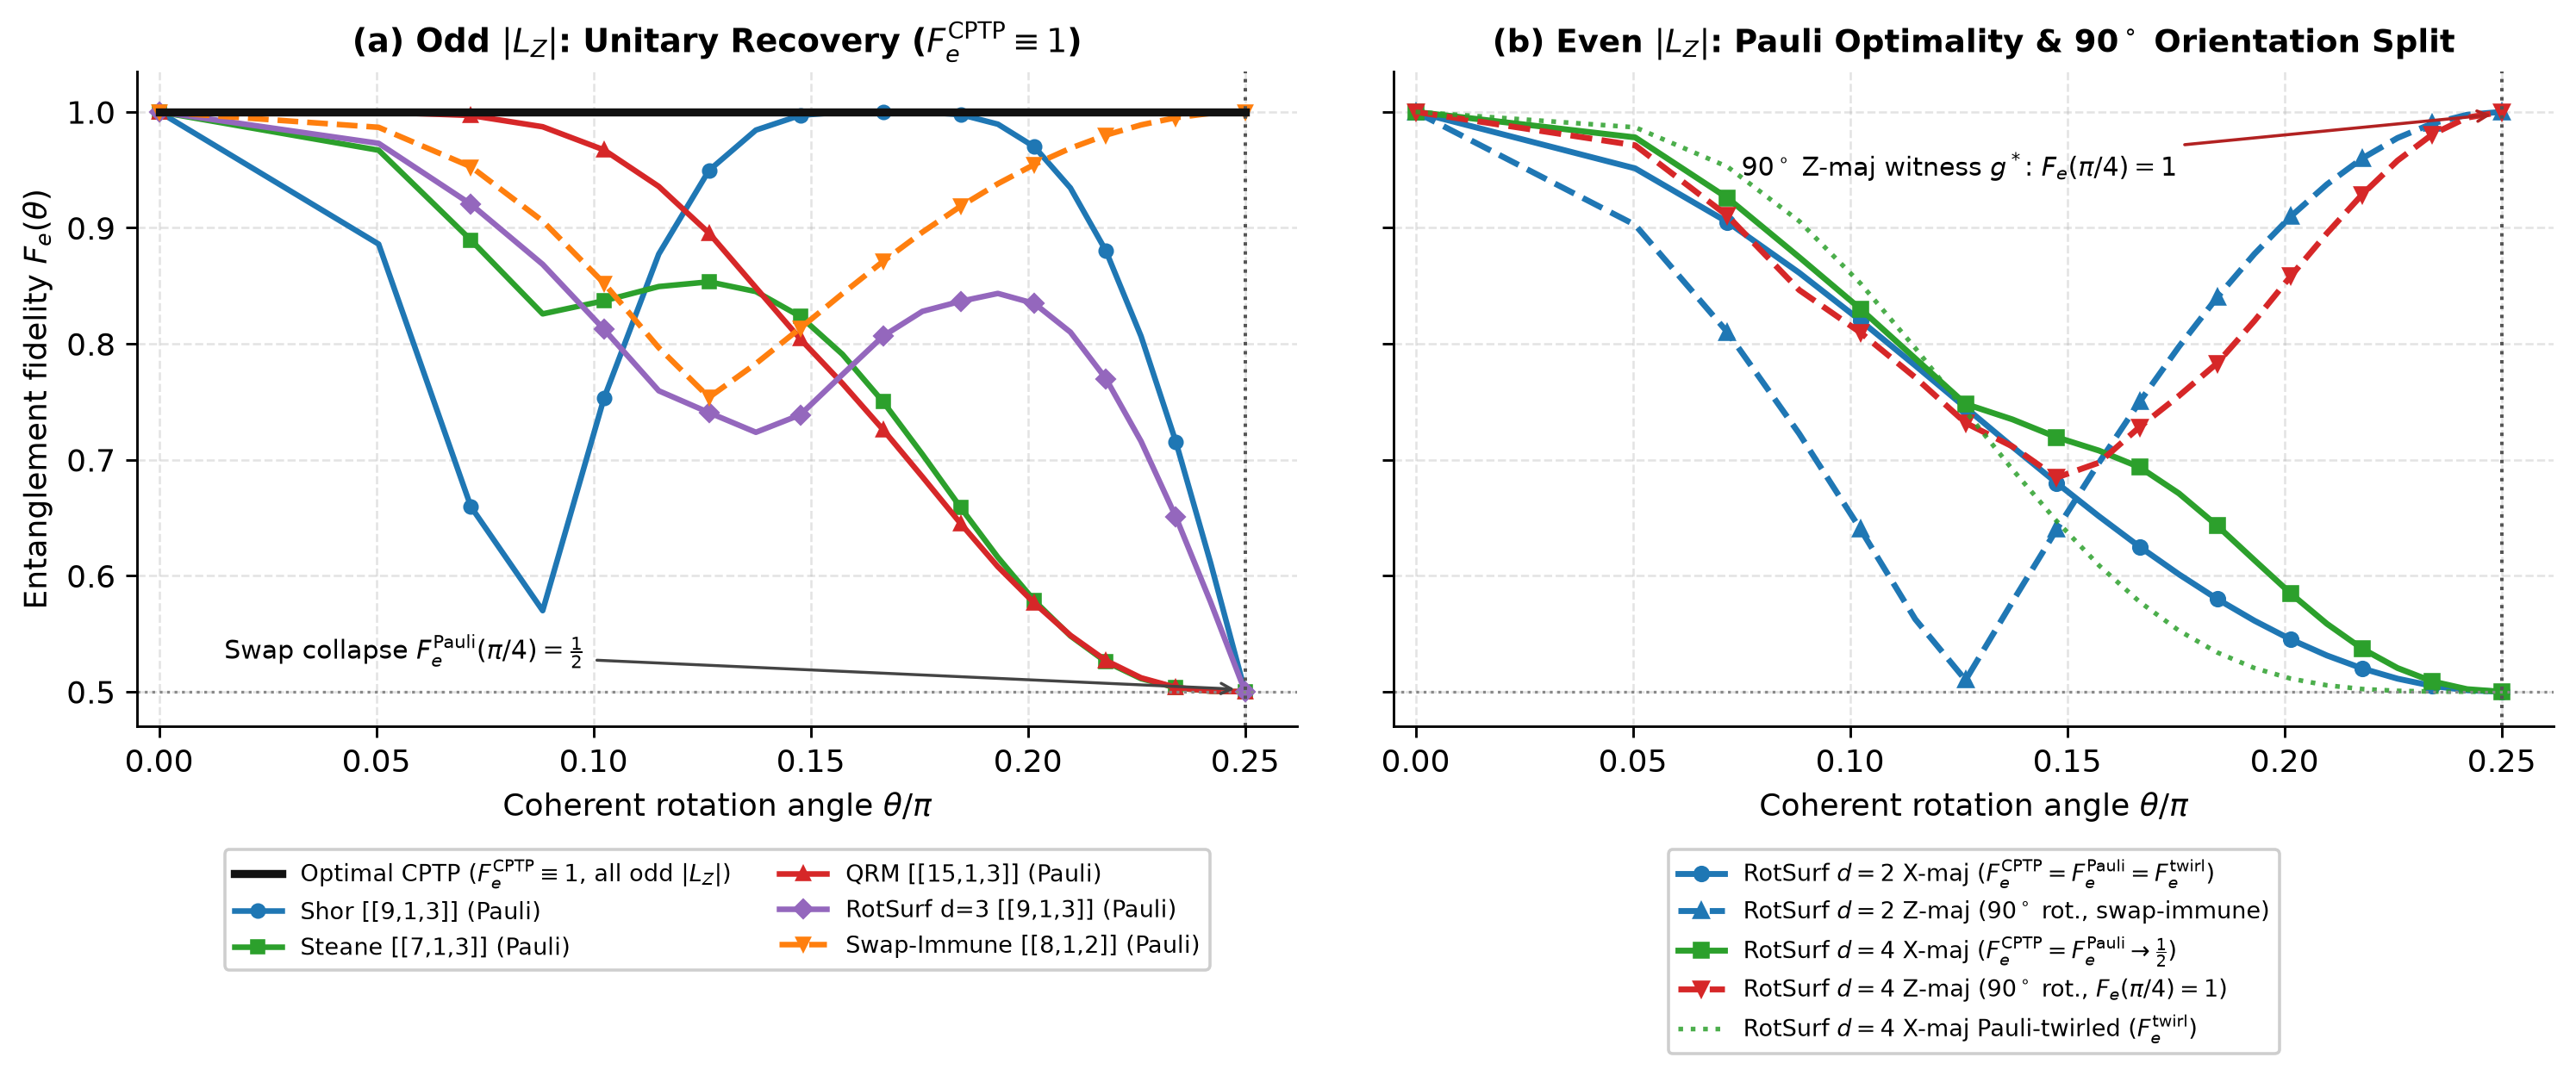
\includegraphics[width=\textwidth]{figures/fig1_parity_dichotomy_curves.png}
  \caption{Exact-$\Q$ entanglement fidelity sweeps across $\theta \in [0,\pi/4]$. (a)~Odd-$|L_Z|$ codes satisfy $F_e^{\mathrm{CPTP}}(\theta) \equiv 1$ identically, while Pauli decoding collapses to $1/2$ when $L_Z \perp \KZ$ or rebounds to $1$ on \texttt{swap\_immune\_8\_1\_2\_odd}. (b)~Even-$|L_Z|$ codes satisfy $F_e^{\mathrm{CPTP}}(\theta) \equiv F_e^{\mathrm{Pauli}}(\theta)$, and a $90^\circ$ patch rotation on $d=2,4$ rotated surface codes flips the $\theta=\pi/4$ limit from $1/2$ ($X$-majority) to $1$ ($Z$-majority).}
  \label{fig:fig1}
\end{figure}

\begin{figure}[t]
  \centering
  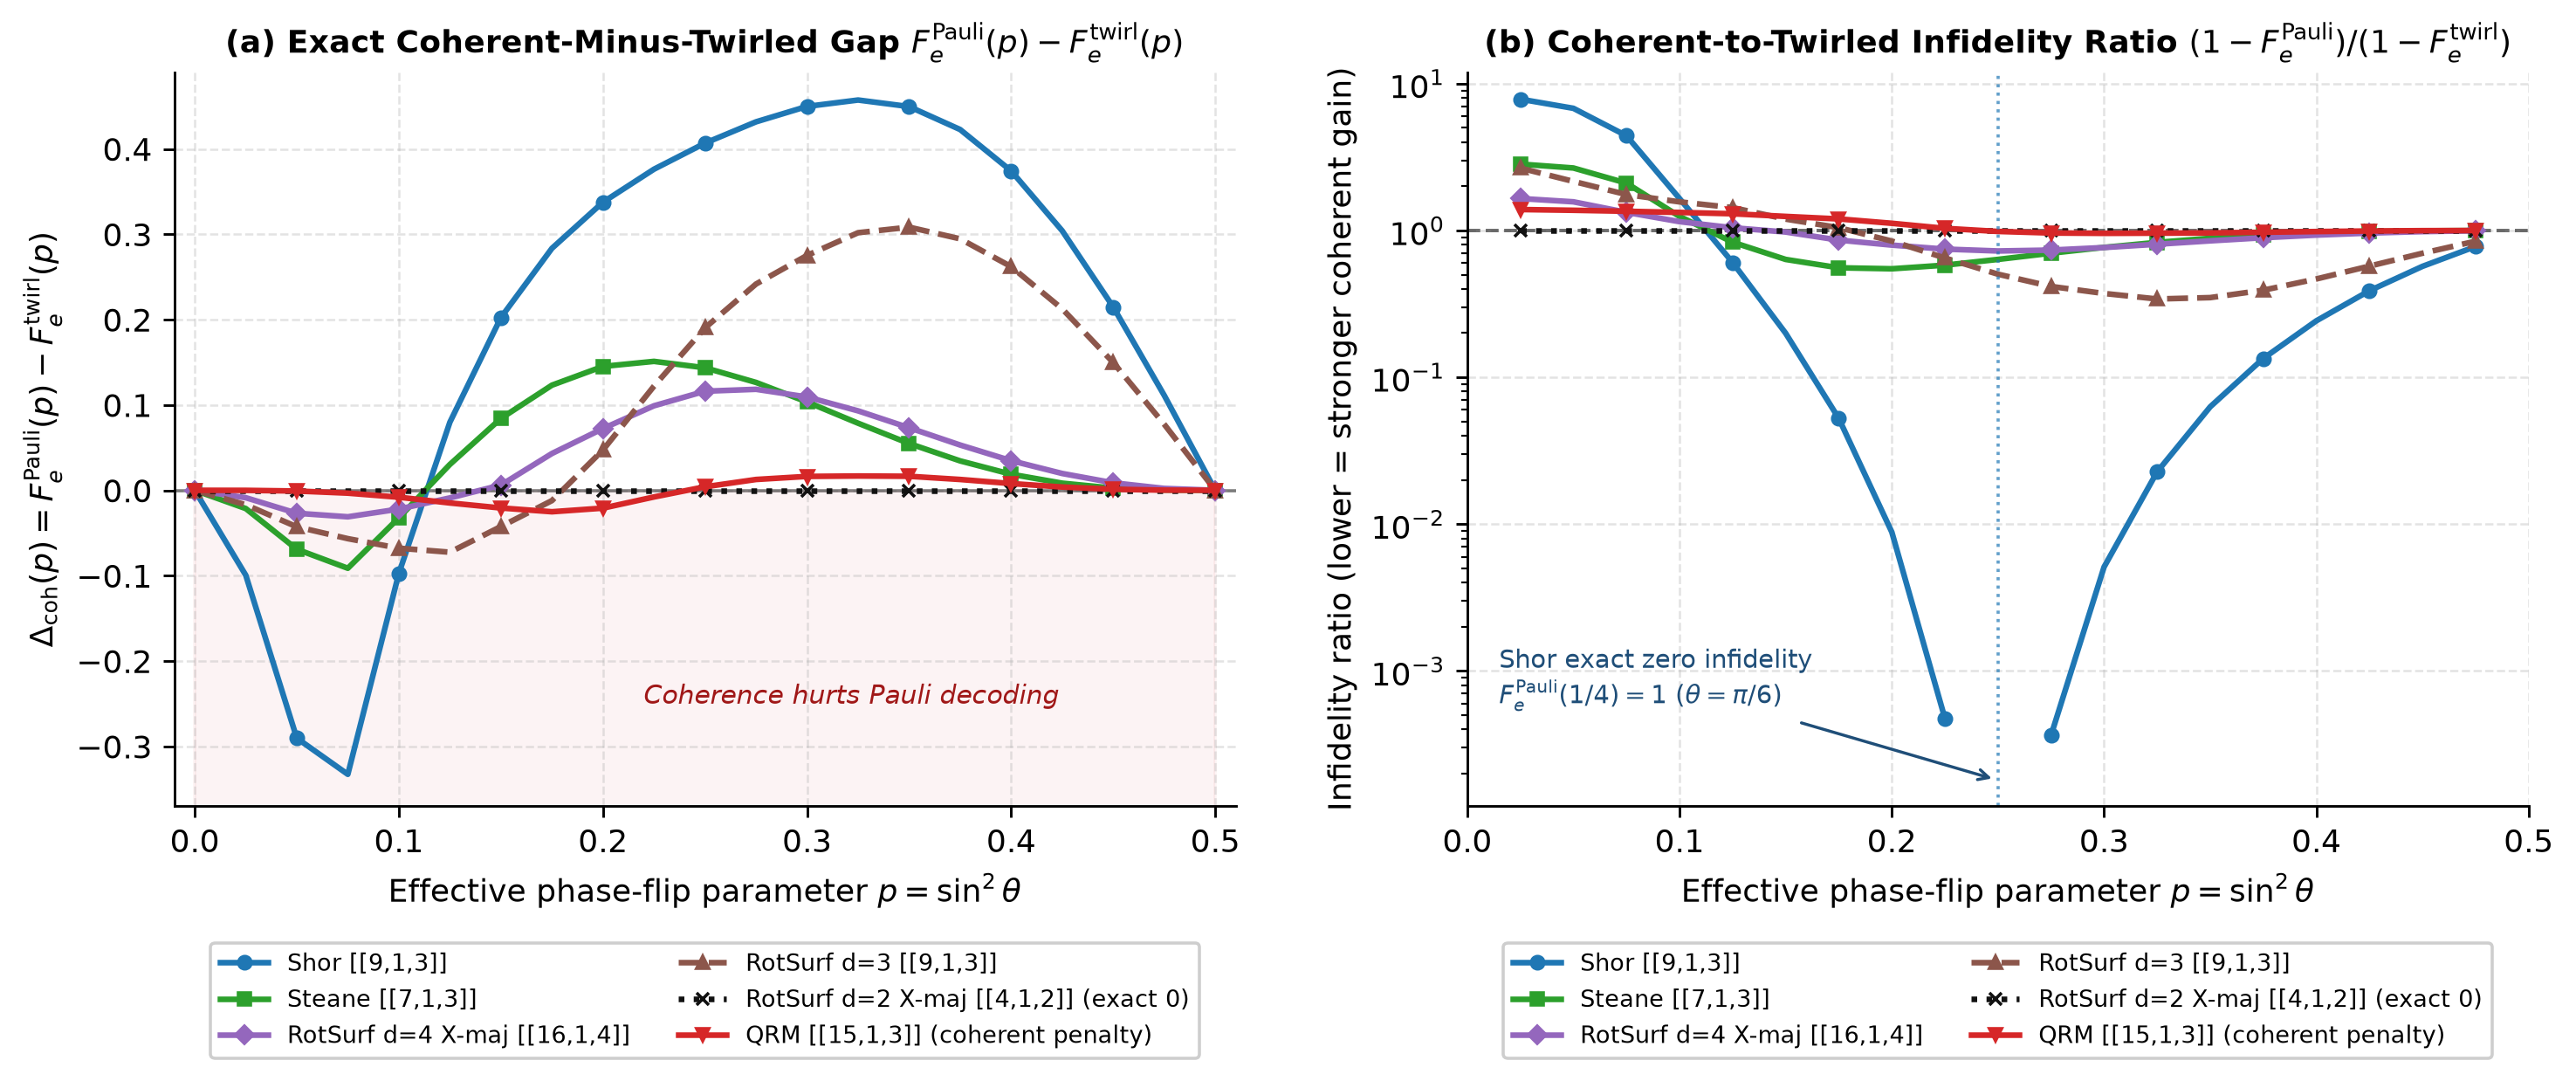
\includegraphics[width=\textwidth]{figures/fig2_coherent_vs_twirled_gap.png}
  \caption{Coherent vs.\ Pauli-twirled decoding gap across $p = \sin^2\theta \in [0, 1/2]$. (a)~Exact difference $\Delta_{\mathrm{coh}}(p) = F_e^{\mathrm{Pauli}}(p) - F_e^{\mathrm{twirl}}(p)$, revealing exact zero cancellation for \texttt{rotsurf\_d2\_Xmaj} and negative coherent-penalty regions for doubly-even QRM~$[[15,1,3]]$ (and at small $p$ for Steane/Shor/surface codes). (b)~Log-scale coherent-to-twirled infidelity ratio highlighting Shor's exact zero-infidelity singularity $F_e^{\mathrm{Pauli}}(1/4) = 1$ at $\theta = \pi/6$.}
  \label{fig:fig2}
\end{figure}

\subsection{Experiments 3 \& 4: 129-Code Binary Swap-Point Census and Distance Sawtooth}

To stress-test Theorem~\ref{thm:swap-binary} beyond structured families, Experiment~3 evaluates the exact $\theta = \pi/4$ Pauli fidelity across all 9 atlas codes plus 120 deterministically sampled even-$\SZ$ $[[n,1,d]]$ CSS codes ($n \in \{4,\dots,9\}$, seed \texttt{20261124}). Every single one of the \textbf{129 codes} matches Theorem~\ref{thm:swap-binary} with \textbf{0 intermediate values} in $(1/2, 1)$: 67 collapse to $1/2$ (40 odd-$|L_Z|$, 27 even-$|L_Z$) and 62 attain exact unit immunity $1$ (31 odd-$|L_Z|$, 31 even-$|L_Z$), populating all four parity-by-swap quadrants (Figure~\ref{fig:fig3}(a)).

Experiment~4 compares rotated surface codes ($d=2,3,4$, both orientations) against phase-flip repetition codes ($d=2,\dots,9$, $H_Z = \emptyset$, $|L_Z|=d$) at $p \in \{1/20, 1/10, 1/5, 3/10, 2/5, 1/2\}$. Even without any $Z$-stabilizers (where $F_e^{\mathrm{Pauli}}(p) \equiv F_e^{\mathrm{twirl}}(p)$), phase-repetition codes display the exact odd--even CPTP sawtooth of Theorem~\ref{thm:parity-dichotomy}: $F_e^{\mathrm{CPTP}}(1/5)$ oscillates between $1$ (odd $d=3,5,7,9$) and $F_e^{\mathrm{Pauli}}(1/5)$ (even $d=2,4,6,8$; Figure~\ref{fig:fig3}(b)).

\begin{figure}[t]
  \centering
  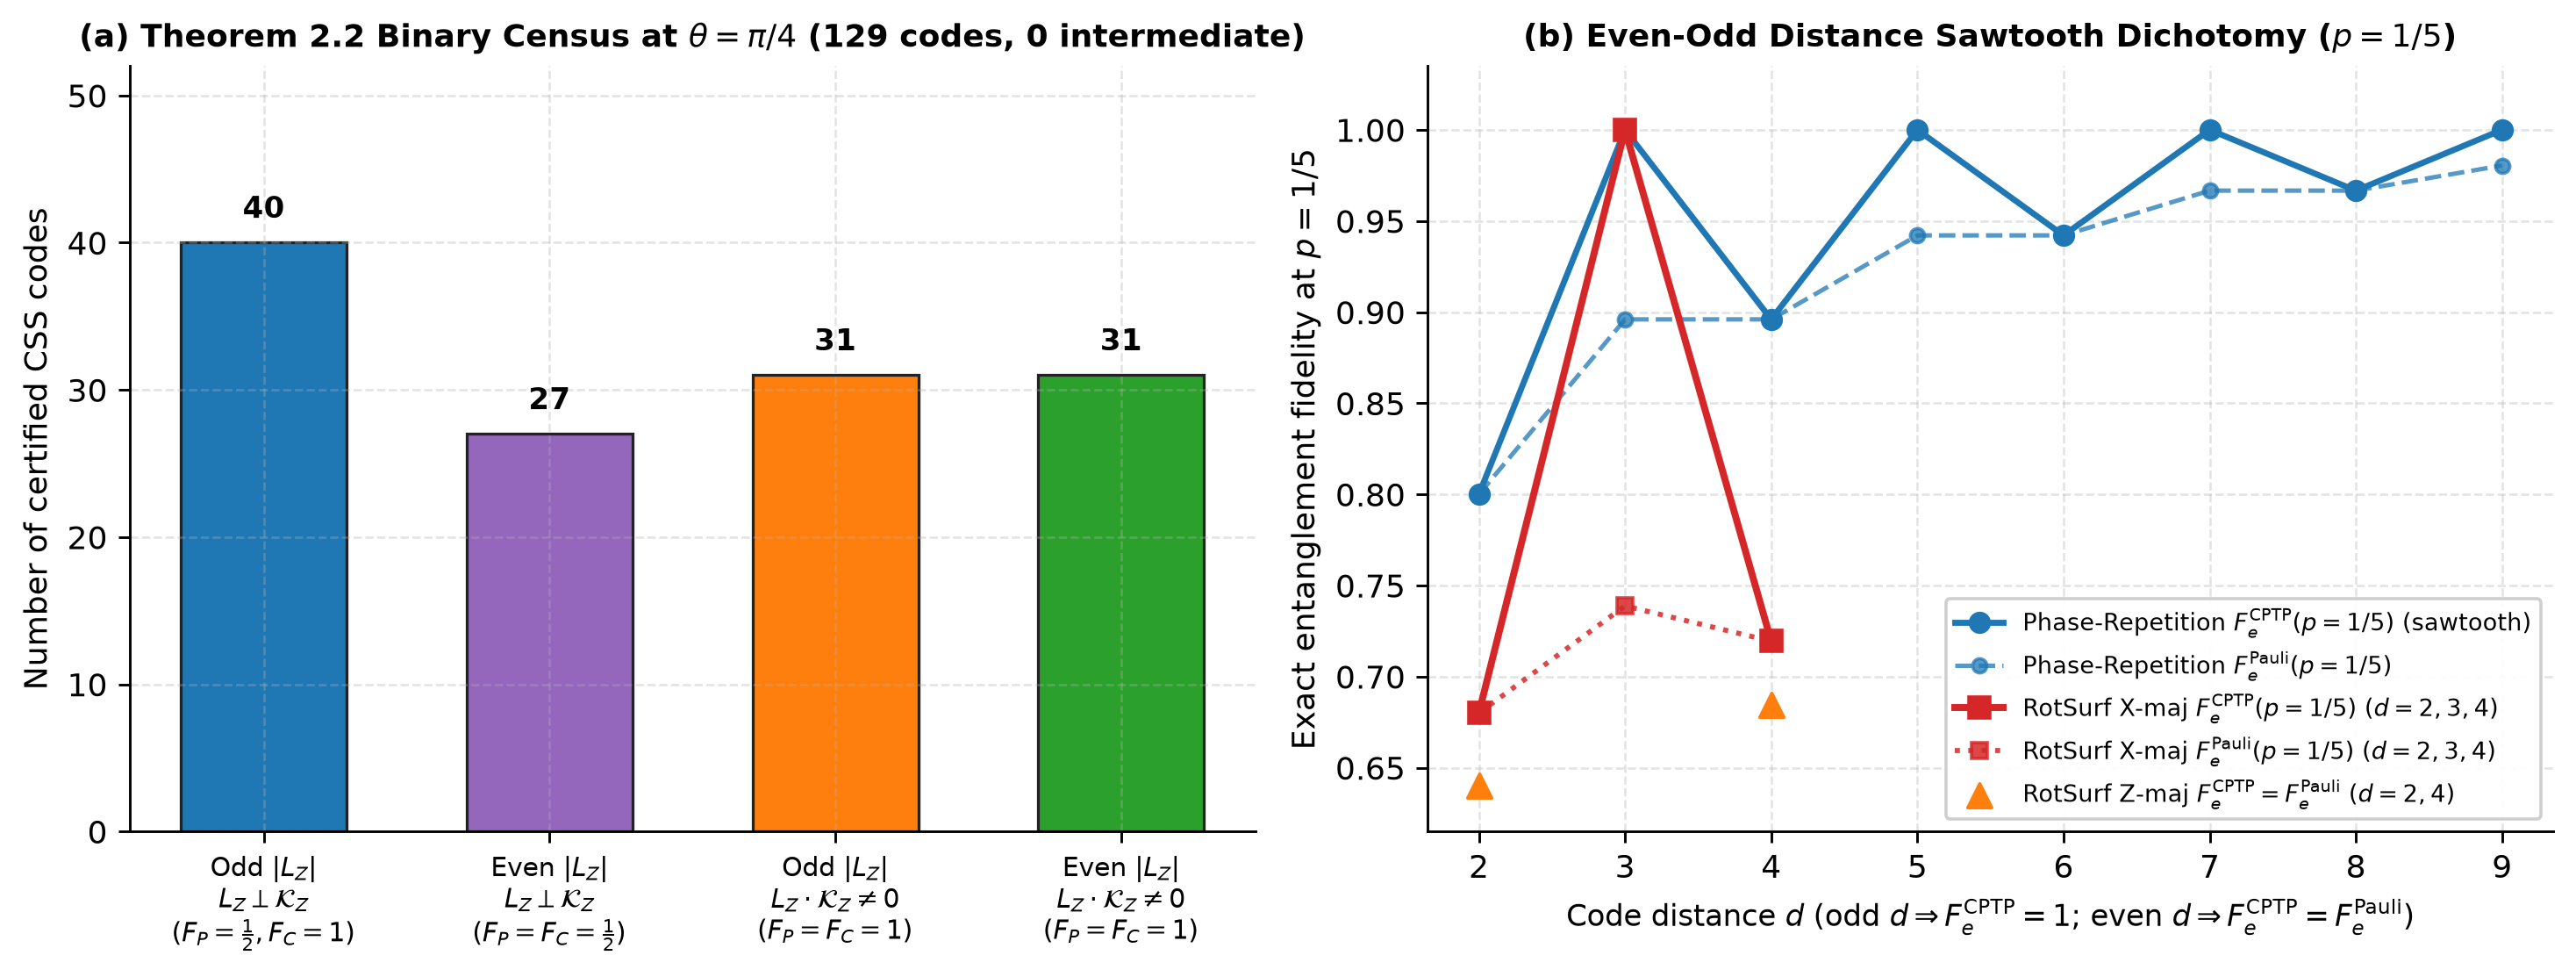
\includegraphics[width=\textwidth]{figures/fig3_swap_point_binary_law.png}
  \caption{(a)~Experiment~3 census across 129 certified CSS codes at $\theta = \pi/4$: all four quadrants of (odd/even $|L_Z|$) $\times$ ($L_Z \perp \KZ$ vs.\ $L_Z \not\perp \KZ$) are populated with 129/129 exact Theorem~\ref{thm:swap-binary} matches and 0 intermediate values in $(1/2, 1)$. (b)~Experiment~4 even--odd distance sawtooth dichotomy at $p = 1/5$ for phase-repetition ($d=2,\dots,9$) and rotated surface ($d=2,3,4$) codes.}
  \label{fig:fig3}
\end{figure}

\subsection{Adversarial Security Audit}

In \texttt{tests/test\_suite.py}, we attack \texttt{verify\_\allowbreak coherent\_\allowbreak css\_\allowbreak certificate\_\allowbreak exact} with \textbf{37 live adversarial payloads} covering bad schema versions, missing or rogue keys at all four dictionary levels, float, \texttt{bool}, \texttt{Decimal}, \texttt{tuple}, non-string-key, and non-string \texttt{code\_name}/\texttt{family} injections, unreduced or non-canonical rationals (\texttt{"2/4"}, \texttt{"1/1"}, \texttt{"+1/2"}, leading whitespace, trailing newlines \texttt{"1/2\textbackslash n"} and \texttt{"1\textbackslash n"}), broken CSS commutativity, odd-weight $H_Z$ rows, trivial logicals, forged parity branches, forged $F_e^{\mathrm{CPTP}} = 1$ on even-$|L_Z|$ \texttt{rotsurf\_d4\_Xmaj}, $10^{-6}$-perturbed fidelities, missing/forged/dependent \texttt{K\_Z\_basis}, missing/forged/spurious swap-immunity witnesses, missing mandatory $p=1/2$ points, and tampered, reversed, non-integer, or duplicated coset enumerators. All \textbf{37/37 attacks are rejected} with explicit \texttt{ValueError} diagnostics.

\section{Scope, Limitations, and Conclusion}

Our exact dichotomy and $0$--$1$ binary law govern uniform coherent $Z$-rotations $U(\theta) = \bigotimes_{j=1}^n e^{i\theta Z_j}$ on $k=1$ CSS codes with even-weight $Z$-stabilizers (with Theorem~\ref{thm:swap-binary} holding even without the even-weight hypothesis). Several natural extensions remain open: (i)~multi-logical $[[n,k,d]]$ CSS codes ($k \ge 2$), where $K_s(\theta)$ acts on $\C^{2^k}$ and the trace-norm optimization becomes a $2^k$-dimensional matrix problem; (ii)~spatially inhomogeneous angles $\{\theta_j\}_{j=1}^n$ or combined coherent $Z$-rotations plus stochastic depolarizing noise, where the exact $F_e^{\mathrm{CPTP}} \equiv 1$ ceiling softens into the finite-size crossover analyzed in~\cite{Dai2026CoherentSurface}; and (iii)~scaling exact rational coset evaluation beyond $n=18$ via tensor-network or Majorana-fermion contraction over exact number fields.

Within the uniform coherent CSS setting, our results provide a complete, machine-checked algebraic classification: the even--odd CPTP optimality dichotomy holds universally across all even-$\SZ$ CSS codes, the $\theta = \pi/4$ Pauli fidelity is strictly quantized to $\{1/2, 1\}$ by $L_Z \perp (\SZ \cap \SZ^\perp)$, and a $90^\circ$ orientation rotation of any even-$d$ rotated surface code flips its maximal-coherence logical survival from $50\%$ to $100\%$. All Lean~4 proofs, Python verifiers, certificates, and SHA-256 manifests are archived at \url{https://github.com/lluiseriksson/coherent-css-dichotomy}.

\bibliographystyle{unsrt}
\bibliography{references}

\end{document}
